\documentclass[11pt, oneside]{article} 
\usepackage{geometry}
\geometry{letterpaper} 
\usepackage{graphicx}
	
\usepackage{amssymb}
\usepackage{amsmath}
\usepackage{parskip}
\usepackage{color}
\usepackage{hyperref}

\graphicspath{{/Users/telliott_admin/Dropbox/Tex/png/}}
% \begin{center} 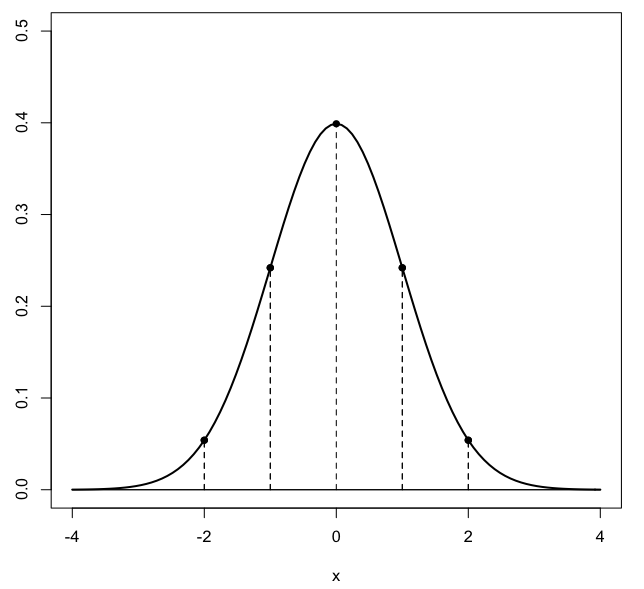
\includegraphics [scale=0.4] {gauss3.png} \end{center}

\title{Proof}
\date{}

\begin{document}
\maketitle
\Large

Imagine a glass cylinder, shown here in cross-section and colored black.  The cylinder has been sliced through at an angle by a plane, and we suppose a flat piece of glass in the shape of an ellipse is glued between the two halves.  

The elongated region in red (formed at the plane of the cut) is the ellipse, and the cylinder is oriented so that at each horizontal position going across the page, the two points on the ellipse are at the same vertical position.  We see the plane of the cut edge-on.
\begin{center} 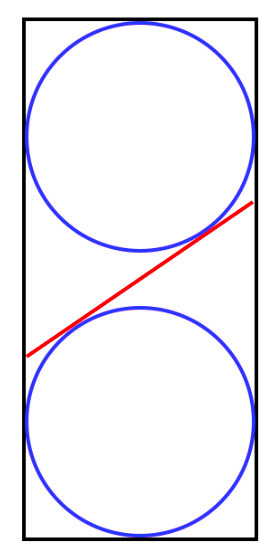
\includegraphics [scale=0.35] {cylinder_slant1.png} \end{center}
Two spheres that fit snugly inside the cylinder lie above and below the ellipse, just touching it.  The planar surface of the ellipse is tangent to the spheres, touching each one at a single point.

We claim that the points where the spheres touch the ellipse are the foci of the ellipse.

By the nature of the construction, the two spheres just fit inside the cylinder.  That means the intersection where the spheres touch the cylinder is a circle, the lower one is shown with a dotted blue line in the next figure.
\begin{center} 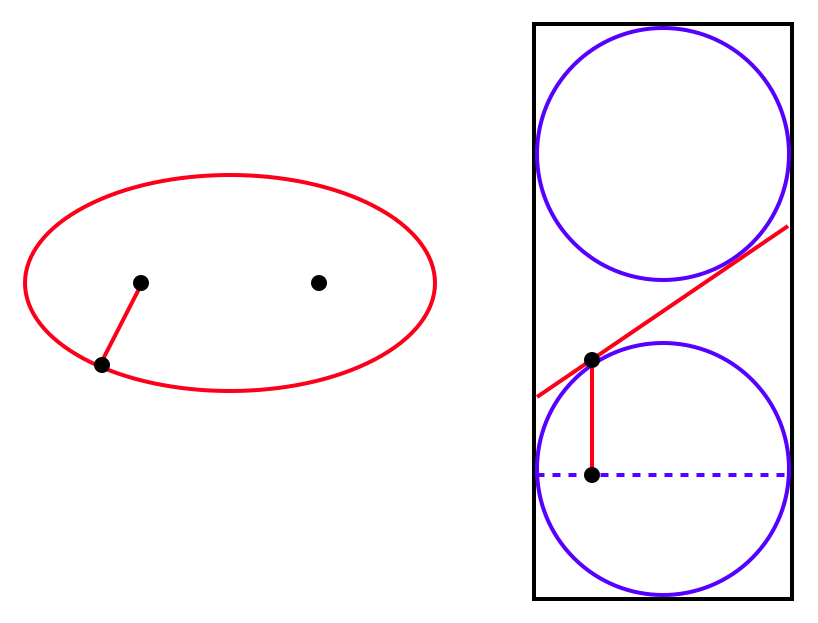
\includegraphics [scale=0.35] {cylinder_slant2.png} \end{center}
Now consider any point on the ellipse.  On the left, we see one point on the ellipse together with two interior points we claim are foci, with a line drawn from our point to one of the foci. 

We said that this point is the point where the ellipse touches the lower sphere.  We conclude that the line we've drawn from the edge of the ellipse to the focus is a tangent to the sphere. 

A second tangent of interest is the perpendicular dropped vertically down the surface of the cylinder, shown in the right panel. Since they are both tangents, this line is the same length as line to the focus.

But the construction, and this equality, holds for any point on the ellipse, as shown in the next figure.
\begin{center} 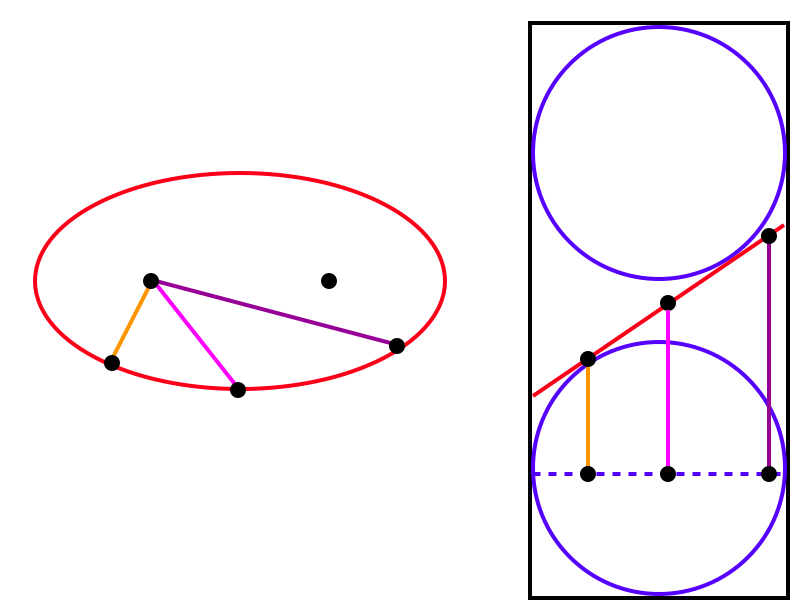
\includegraphics [scale=0.35] {cylinder_slant3.png} \end{center}
Finally, this is true for both spheres (below). The sum of the perpendicular tangents for any point is a constant. 
\begin{center} 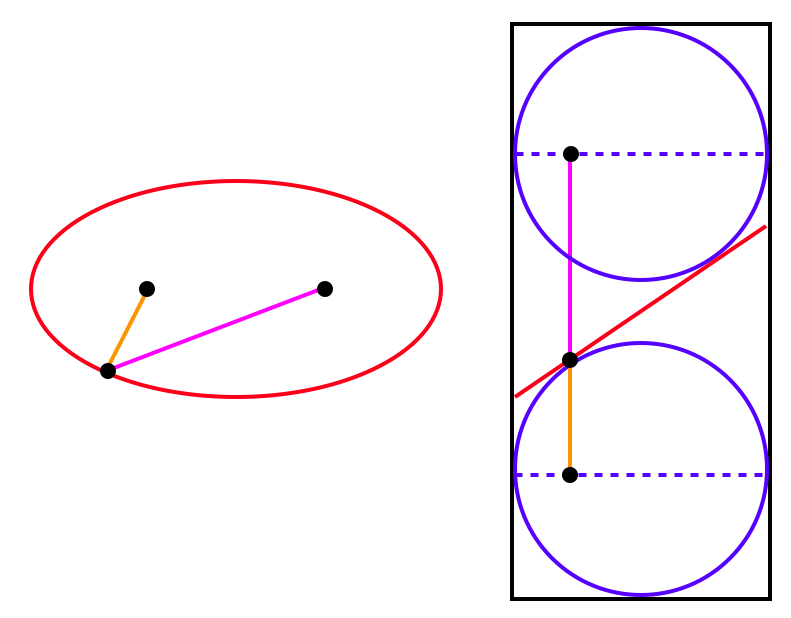
\includegraphics [scale=0.35] {cylinder_slant4.png} \end{center}
Thus, the points where the spheres touch the ellipse are its foci, because the sum of the distances to any point on the ellipse, which is equal to the sum of the vertical tangents, is a constant.


\end{document}